\documentclass[journal]{vgtc}                     % final (journal style)
%\documentclass[journal,hideappendix]{vgtc}        % final (journal style) without appendices
%\documentclass[review,journal]{vgtc}              % review (journal style)
%\documentclass[review,journal,hideappendix]{vgtc} % review (journal style)
%\documentclass[widereview]{vgtc}                  % wide-spaced review
%\documentclass[preprint,journal]{vgtc}            % preprint (journal style)

\onlineid{0}

\vgtccategory{Research}

%% Paper title.
\title{A Configurable Street-Level Vision Node for Curio: Bringing Pre-Trained CV into Urban Visual Analytics Workflows}

\author{%
  L.~Sravya Rachakonda \hspace{2.5em} Laxmi Sai Maneesh Reddy Jupalle
  \\[4pt]
  \normalfont University of Illinois at Chicago
}

%% Author footer disabled per request. Restore by uncommenting if VGTC reviewers require affiliations.
%\authorfooter{
%  \item
%    L.~Sravya Rachakonda is with the University of Illinois Chicago.
%    E-mail: lrach3@uic.edu.
%  \item
%    Laxmi Sai Maneesh Reddy Jupalle is with the University of Illinois Chicago.
%    E-mail: ljupa2@uic.edu.
%}
\authorfooter{}

%% Suppress the bottom-of-first-page IEEE boilerplate
%% (manuscript-received line + Digital Object Identifier line).
\renewcommand{\manuscriptnotetxt}{}
\nocopyrightspace

%% Suppress the decorative diamond-rule separator between abstract and body.
\renewcommand{\diamondrule}{}
\let\diamondrule\relax

%% Suppress the page-header rule on continuation pages.
\renewcommand{\headrule}{}
\renewcommand{\headrulewidth}{0pt}

\abstract{%
  Urban analysts increasingly want to derive block-level signals (greenery, sidewalk coverage, vehicle composition, accessibility infrastructure) from street-level imagery, but the existing path requires custom Python scripts, model loading boilerplate, and ad-hoc spatial joins that put computer vision (CV) out of reach for non-programmers. We extend Curio, a node-based urban visual analytics platform, with a two-node CV pipeline: a \emph{Street Vision} node that performs place-name search, Google Street View sampling, and pre-trained model inference, and a \emph{CV Analysis} node that handles result inspection, per-class metrics, neighborhood enrichment, and GeoJSON/DataFrame export to downstream Vega-Lite and UTK nodes. Users select any HuggingFace segmentation or detection checkpoint via the in-node search; our demo uses Mask2Former-Swin-Large on Cityscapes for segmentation and supports YOLOv8 for detection. We demonstrate the system on a Chicago greenery assessment and a vehicle-counting case study, document seven newly enabled analytical tasks, and report representative inference latency on CPU. The paper closes with limitations around demo-mode batch caps, the fixed Cityscapes taxonomy, and the spatial sparsity of Street View metadata coverage.
}

\keywords{Urban visual analytics, dataflow systems, semantic segmentation, street-level imagery, Curio.}

\teaser{
  \centering
  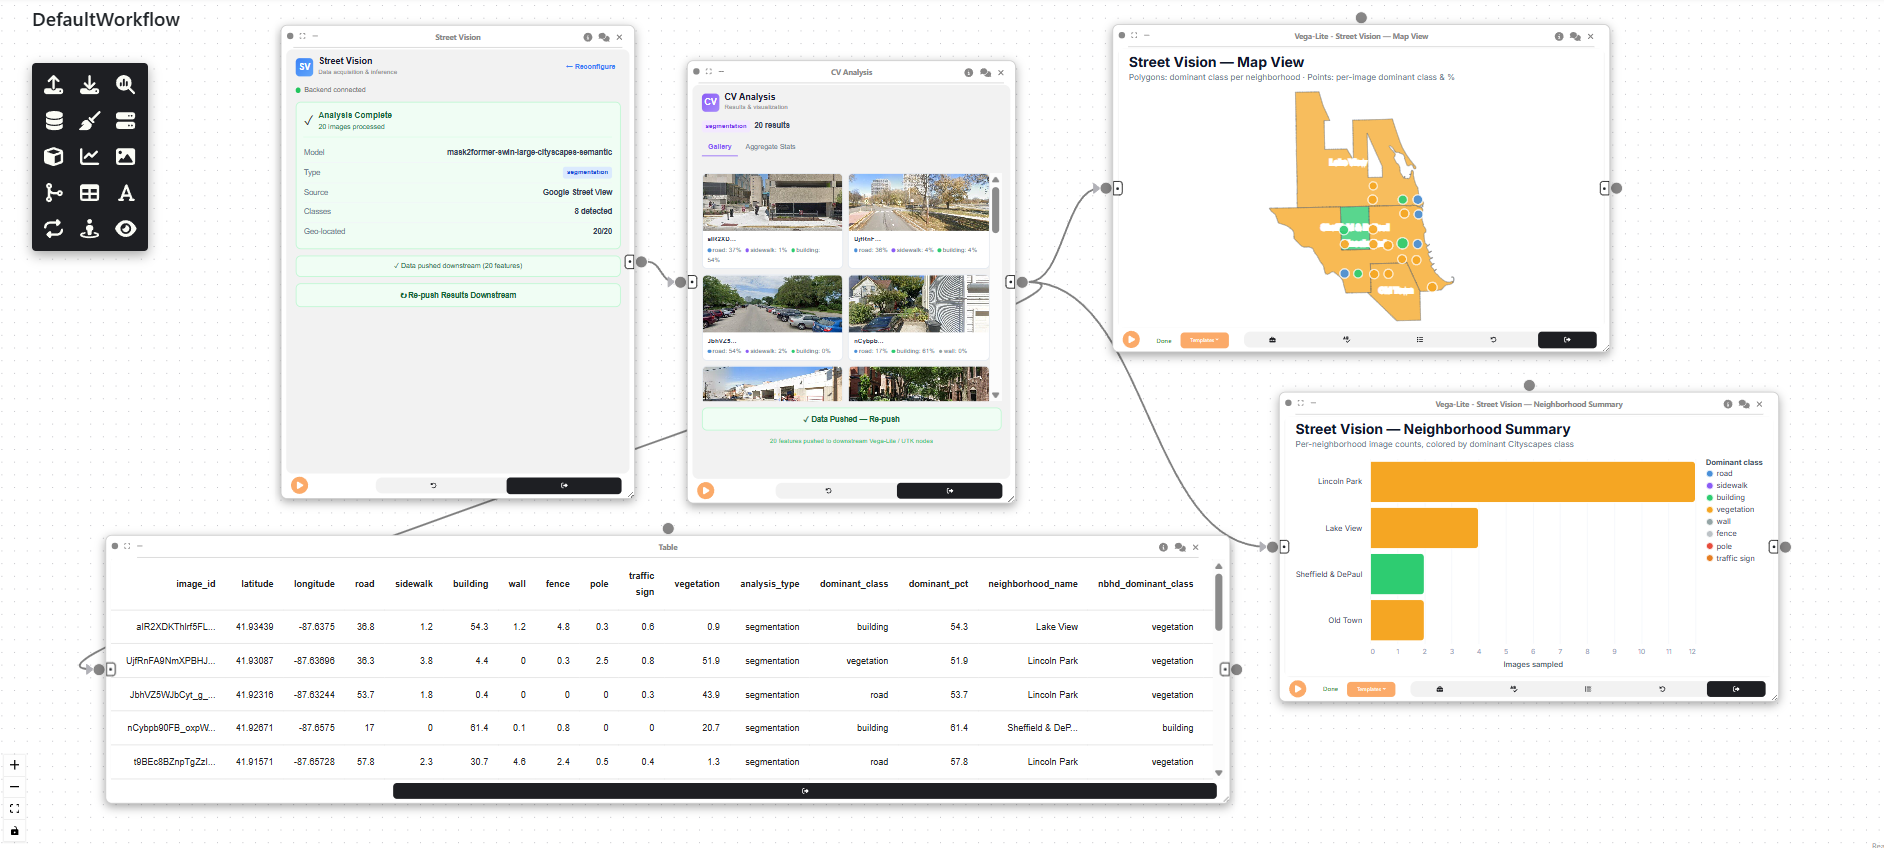
\includegraphics[width=\linewidth, alt={Curio canvas showing a Street Vision node connected to a CV Analysis node, which fans out to a Vega-Lite Map View of Chicago neighborhoods, a per-neighborhood summary bar chart, and a tabular view of all per-image features.}]{teaser_curio_canvas}
  \caption{%
    The Street-Level Vision Analytics extension on the Curio canvas. A \emph{Street Vision} node (place search, model selection, inference) feeds a \emph{CV Analysis} node, which emits a GeoJSON FeatureCollection enriched with Chicago neighborhood polygons. Three downstream consumers read different projections of the same payload: a Vega-Lite Map View coloured by modal Cityscapes class, a Vega-Lite Neighborhood Summary bar chart of per-neighborhood image counts, and a Table node exposing the per-image feature row.%
  }
  \label{fig:teaser}
}

%%%%%%%%%%%%%%%%%%%%%%%%%%%%%%%%%%%%%%%%%%%%%%%%%%%%%%%%%%%%%%%%
%%%%%%%%%%%%%%%%%%%%%% LOAD PACKAGES %%%%%%%%%%%%%%%%%%%%%%%%%%%
%%%%%%%%%%%%%%%%%%%%%%%%%%%%%%%%%%%%%%%%%%%%%%%%%%%%%%%%%%%%%%%%

\graphicspath{{figs/}{figures/}{pictures/}{images/}{./}}

\usepackage{tabu}
\usepackage{booktabs}
\usepackage{ccicons}
\usepackage{mathptmx}

\begin{document}

\firstsection{Introduction}

\maketitle

Cities now publish or stream petabyte-scale street-level imagery (Google Street View, Mapillary, municipal LiDAR rigs), and a decade of computer-vision research has shown that pre-trained semantic segmentation and object detection models can extract policy-relevant signals from those images: tree canopy~\cite{Li2015AssessingStreetlevelUrban}, sidewalk condition, vehicle composition~\cite{Gebru2017UsingDeepLearning}, and pedestrian infrastructure. The catch is workflow friction. An urban planner asking ``which Lincoln Park blocks have less than 10\% sidewalk?'' has to learn HuggingFace's API~\cite{Wolf2020TransformersStateoftheartNatural}, write image-fetching code against the Street View Static API, manage a CUDA environment, run inference, then stitch the results into a GIS workflow alongside census tracts. The CV is the easy part; the plumbing is what blocks adoption.

Node-based visual analytics platforms such as Curio~\cite{Moreira2024CurioDataflowFramework} and KNIME~\cite{Berthold2009KNIMEKonstanzInformation} were designed to remove exactly this kind of plumbing for tabular and geospatial workflows, but none of them ship a node that runs a pre-trained CV model on live street imagery. We close that gap. Our contribution is a \emph{two-node} extension to Curio that handles model selection, place-name search, Street View sampling, inference, neighbourhood enrichment, and export to Vega-Lite and UTK, all behind a configuration UI that exposes no Python (\autoref{fig:teaser}). Concretely we contribute (1) a \textbf{Street Vision} node that wraps HuggingFace model search and Google Street View sampling behind a place-name interface, (2) a \textbf{CV Analysis} node that performs server-side spatial joins against Chicago neighborhood polygons and emits both GeoJSON and DataFrame outputs, and (3) a Curio-native Vega-Lite \emph{Map View} template that renders neighborhoods coloured by their modal Cityscapes class. We evaluate via a seven-task analytical inventory and two case studies (Chicago greenery; vehicle counting in The Loop).

\section{Related Work}
\label{sec:related}

\textbf{Urban visual analytics platforms.} Curio~\cite{Moreira2024CurioDataflowFramework} introduced a dataflow abstraction for urban analytics that lets analysts wire together data acquisition, transformation, and visualization nodes; the underlying Urban Toolkit (UTK)~\cite{Moreira2023UrbanToolkitGrammar} provides a grammar for thematic urban maps. These platforms benefit from interactive, multi-view design but historically treat CV outputs as pre-computed inputs rather than a node in the live graph. Our work integrates the inference step itself into the graph.

\textbf{Street-level imagery analysis.} Prior work uses street-level imagery to infer block- or neighborhood-scale attributes: Treepedia~\cite{Li2015AssessingStreetlevelUrban} estimated street-level greenery from Google Street View at city scale, and Gebru et al.~\cite{Gebru2017UsingDeepLearning} used vehicle make/model recognition over 50M Street View images to infer demographics. These studies are typically one-off pipelines in research code; we package the workflow as reusable nodes so non-programmers can re-run the same kind of analysis on new bounding boxes or with substituted models.

\textbf{Pre-trained CV for cities.} SegFormer~\cite{Xie2021SegFormerSimpleEfficient} achieves state-of-the-art accuracy on the Cityscapes 19-class urban benchmark~\cite{Cordts2016CityscapesDatasetSemantic}, and YOLOv8~\cite{Jocher2023YOLOv8} provides fast object detection on commodity CPUs. The HuggingFace Hub~\cite{Wolf2020TransformersStateoftheartNatural} aggregates thousands of such checkpoints; we expose the Hub's search API directly inside the Street Vision node so users can swap models without code changes. We treat the transferability of Cityscapes-trained models to U.S. street imagery as a working assumption rather than a contribution.

\textbf{No-code visual analytics.} Vega-Lite~\cite{Satyanarayan2017VegaLiteGrammarInteractive}, KNIME~\cite{Berthold2009KNIMEKonstanzInformation}, and Tableau define the modern expectation that data analysts work without writing imperative code. Our extension follows that tradition: every parameter the user might want to change (model, location, target classes, filtering operator) is a UI control, not a Python edit. The heavy work (CV inference) happens server-side and only the resulting GeoJSON is shipped to the client.

\section{Data and Tasks}
\label{sec:data}

\textbf{Imagery.} We consume images from the Google Street View Static API and use the companion Metadata API for free coverage probing before any paid request. A user-supplied place name (e.g.~``Lincoln Park Chicago'') is geocoded by OpenStreetMap Nominatim into a bounding box; the box is sampled on a regular grid; each sample is checked against the Metadata API; covered samples are then fetched as 640$\times$480 images at 90$^{\circ}$ field of view. The sampling density and per-request cap are configurable on the Street Vision node.

\textbf{Spatial reference.} For Chicago we ship a curated GeoJSON of 98 neighborhood polygons, indexed in memory with a Shapely STRtree so that point-in-polygon joins for hundreds of inference results complete in well under a second. Each result feature is tagged with its neighborhood name, and per-neighborhood roll-ups (modal class, mean dominance percentage, image count) are computed server-side and exposed at \texttt{/api/data/basemap/enrich\_with\_neighborhoods}.

\textbf{Models.} The system has no hardcoded default model. The user picks any HuggingFace semantic segmentation or detection checkpoint via the in-node search, with the option of auto-picking the top result by download count for a given query. The backend's loader is architecture-agnostic: it tries \texttt{AutoModelForSemanticSegmentation}, then \texttt{AutoModelForUniversalSegmentation}, then \texttt{AutoModelForInstanceSegmentation}, so SegFormer, BEiT, and DPT load through the first path while MaskFormer, Mask2Former, and OneFormer load through the universal path. Our case study below uses \texttt{facebook/mask2former-swin-large-cityscapes-semantic}, the top auto-pick result for the query ``cityscapes'' on the day of the demo, predicting the standard 19-class Cityscapes taxonomy. For object detection we use \texttt{ultralytics/yolov8n} for the vehicle-counting case study.

\textbf{Tasks.} \autoref{tab:tasks} summarizes seven analytical tasks the node enables; full descriptions, target user roles, and ``how it was done before'' baselines are documented in the project repository. The tasks span environmental equity (greenery, seasonal vegetation), pedestrian infrastructure (sidewalk coverage, ramps, street furniture), and verification workflows (manual CV inspection). The two case studies in \autoref{sec:eval} cover tasks 1 and (in spirit) 2.

\begin{table}[tb]
  \caption{Seven analytical tasks newly enabled by the node, by representative model class and primary metric. Time-savings estimates compare the node's interactive workflow against the manual or scripted baselines documented in the project's task inventory.}
  \label{tab:tasks}
  \scriptsize
  \centering
  \begin{tabu} to \columnwidth {@{}c X[l] l l@{}}
    \toprule
    \# & Task & Model class & Primary metric \\
    \midrule
    1 & Compare greenery across neighborhoods    & semantic seg.\ & vegetation ratio \\
    2 & Identify blocks with no street furniture & detection      & furniture count \\
    3 & Verify a CV result against the photo     & any            & visual + bar \\
    4 & Find blocks with poor sidewalk coverage  & semantic seg.\ & sidewalk / road \\
    5 & Audit accessibility ramp presence        & detection      & ramp count \\
    6 & Track seasonal vegetation change         & semantic seg.\ & seasonal delta \\
    7 & Correlate CV metrics with census tracts  & either         & cross-dataset \\
    \bottomrule
  \end{tabu}
\end{table}

\section{System Design}
\label{sec:system}

\textbf{Two-node split.} An early prototype crammed all of model loading, fetching, inference, and visualization into one Curio node; this collapsed Curio's dataflow story into a black box and was rejected after instructor feedback. The shipped design splits computation across two nodes (\autoref{fig:architecture}). The \emph{Street Vision} node owns model selection, place search, sampling, and inference, and emits a structured JSON payload. The \emph{CV Analysis} node consumes that payload, runs the spatial-enrichment join, exposes the gallery / inspector / filter UI, and publishes a GeoJSON \texttt{FeatureCollection} on its output port (a column-oriented DataFrame projection of the same data is reachable via a separate REST endpoint for headless consumers). Downstream Vega-Lite and UTK nodes can be wired to that output without knowing anything about the upstream model.

\begin{figure}[tb]
  \centering
  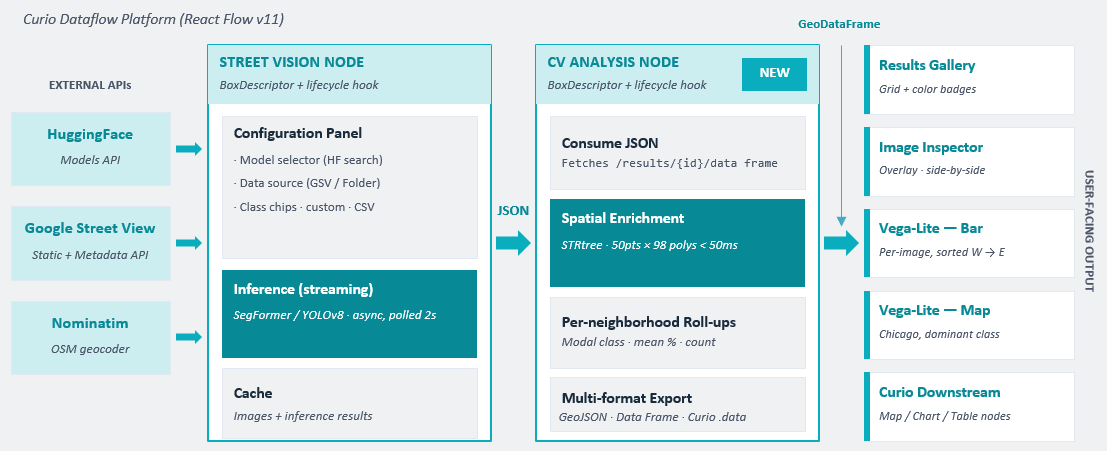
\includegraphics[width=\columnwidth, alt={Architecture diagram showing the Street Vision node's interaction with HuggingFace, Nominatim, and Google Street View, and its handoff to the CV Analysis node, which performs spatial enrichment and feeds Vega-Lite Map View, Vega-Lite bar chart, and Table nodes.}]{architecture}
  \caption{System architecture. Place name $\rightarrow$ Nominatim $\rightarrow$ bounding box $\rightarrow$ Street View Metadata API (coverage check) $\rightarrow$ Street View Static API (image fetch) $\rightarrow$ HuggingFace model inference $\rightarrow$ CV Analysis (Shapely STRtree enrichment) $\rightarrow$ GeoJSON / DataFrame outputs $\rightarrow$ downstream Vega-Lite, Table, and UTK nodes.}
  \label{fig:architecture}
\end{figure}

\textbf{Configuration UI (\autoref{fig:config}).} The Street Vision sidebar is a three-step wizard: (1) model search, (2) data source, and (3) target classes. Each step has sensible defaults so a first-time user can run an analysis in under a minute. Model search hits the live HuggingFace API and is filtered by task type (segmentation or detection); class chips come pre-populated from the Cityscapes 19-class CSV but accept free-text input and CSV uploads for custom taxonomies. The data-source step supports both Street View and a local-folder fallback for offline use.

\begin{figure*}[tb]
  \centering
  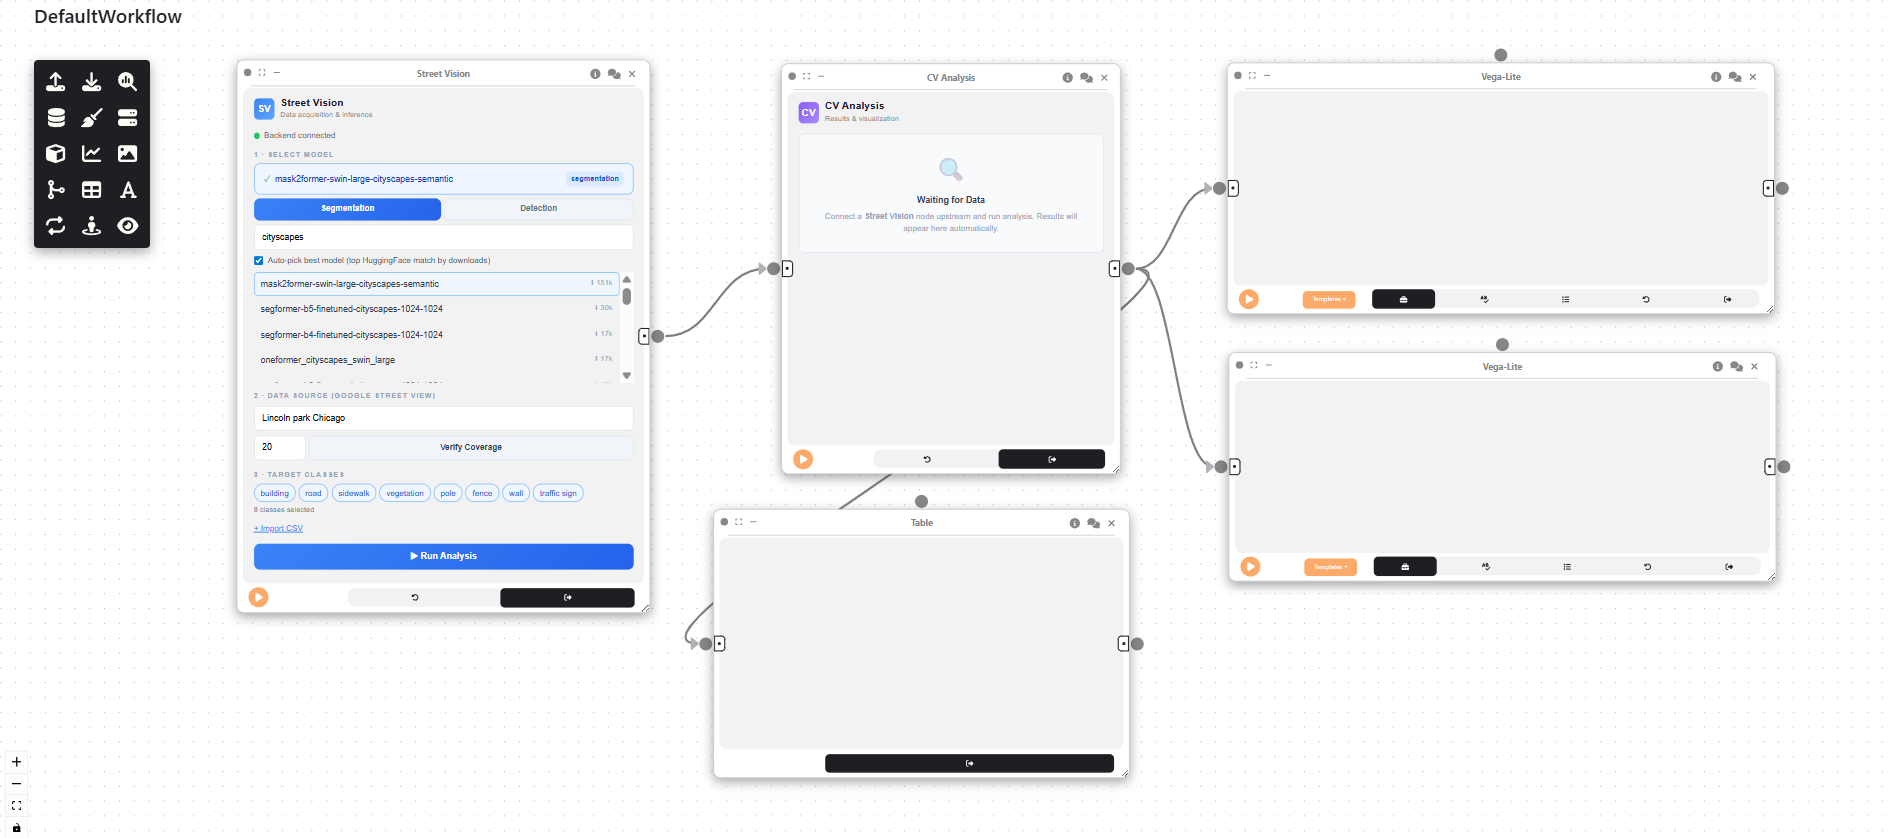
\includegraphics[width=\textwidth, alt={The Street Vision configuration wizard expanded inside the Curio canvas, showing the three-step UI: a HuggingFace model search returning Mask2Former, SegFormer, and OneFormer cityscapes checkpoints with download counts; a data-source step with the place-name input set to Lincoln Park Chicago and a Verify Coverage button; and a target-class chip selector with eight Cityscapes classes selected. A Run Analysis button anchors the bottom.}]{config_wizard}
  \caption{The Street Vision node's three-step configuration wizard, ready to run. Step~1 lists live HuggingFace results sorted by downloads; Step~2 takes a place name and a sample limit; Step~3 exposes Cityscapes class chips plus a CSV upload affordance. The downstream CV~Analysis node sits idle with ``Waiting for Data'' until the user hits \emph{Run Analysis}.}
  \label{fig:config}
\end{figure*}

\textbf{Inference pipeline.} On submit, the backend (a) loads the selected model into a process-wide cache so repeated runs amortize the load cost, (b) batches images through the model on CPU, (c) for segmentation, computes per-pixel class predictions and writes both a logits-derived overlay PNG and a per-class pixel-ratio dictionary, and (d) returns a job id that the frontend polls for status and final results. As a representative reference point, our benchmark runs of SegFormer-B2 at the model's native 1024$\times$1024 input averaged 0.30~s per image on a 4-core CPU. Mask2Former-Swin-Large is a substantially larger checkpoint and was used only for the visual case study, not for latency benchmarking.

\textbf{Spatial enrichment.} The CV Analysis node sends the inference results to \texttt{/api/data/basemap/enrich\_with\_neighborhoods}, which (1) constructs a Shapely \texttt{Point} per result in the basemap's native WGS84, (2) does a single STRtree point-in-polygon query per point, (3) groups by neighborhood and computes per-neighborhood modal class, mean dominance percentage, and image count, and (4) returns both the per-point tags and the per-neighborhood aggregates in one response. Doing this server-side keeps the Vega-Lite and UTK clients stateless: they only see a GeoJSON ready to render.

\textbf{Map View template.} A built-in Vega-Lite spec, selectable from the Vega-Lite node's template menu, paints each searched neighborhood with the colour of its modal class, labels it with the neighborhood name, and overlays per-image points sized by dominance percentage. The same colour palette is shared across the segmentation overlay, the per-class bar chart in the inspector, and the Map View, so a building (green) on the canvas is the same green in the chart and on the map.

\textbf{Implementation.} Backend: Python 3.10, FastAPI, Transformers, Ultralytics, GeoPandas, Shapely. Frontend: React~18 with TypeScript and Vite. Curio integration: a forked Curio repo with two new \texttt{BoxDescriptor} entries and matching React lifecycle hooks; the diff is shipped as a single \texttt{curio-fork.patch}. Total project outside the Curio fork: $\sim$1.8k lines of TypeScript and $\sim$1.6k lines of Python.

\section{Evaluation}
\label{sec:eval}

\textbf{Case study 1: Chicago greenery (\autoref{fig:gallery}).} We ran Mask2Former-Swin-Large fine-tuned on Cityscapes against Street View samples from a Lincoln Park bounding box, with target classes \{vegetation, road, building, sidewalk, sky\}. The Map View renders Lincoln Park (and any other searched neighborhoods) coloured by its modal class; the Neighborhood Summary bar chart, sorted by image count, makes the gradient between residential blocks (more vegetation) and arterial corridors (more road) immediately visible. Compound filters (e.g.~\texttt{vegetation < 0.10}) surface candidate blocks for tree-planting prioritization without any code. The same workflow re-runs identically on Hyde Park or The Loop by typing a new place name.

\begin{figure*}[tb]
  \centering
  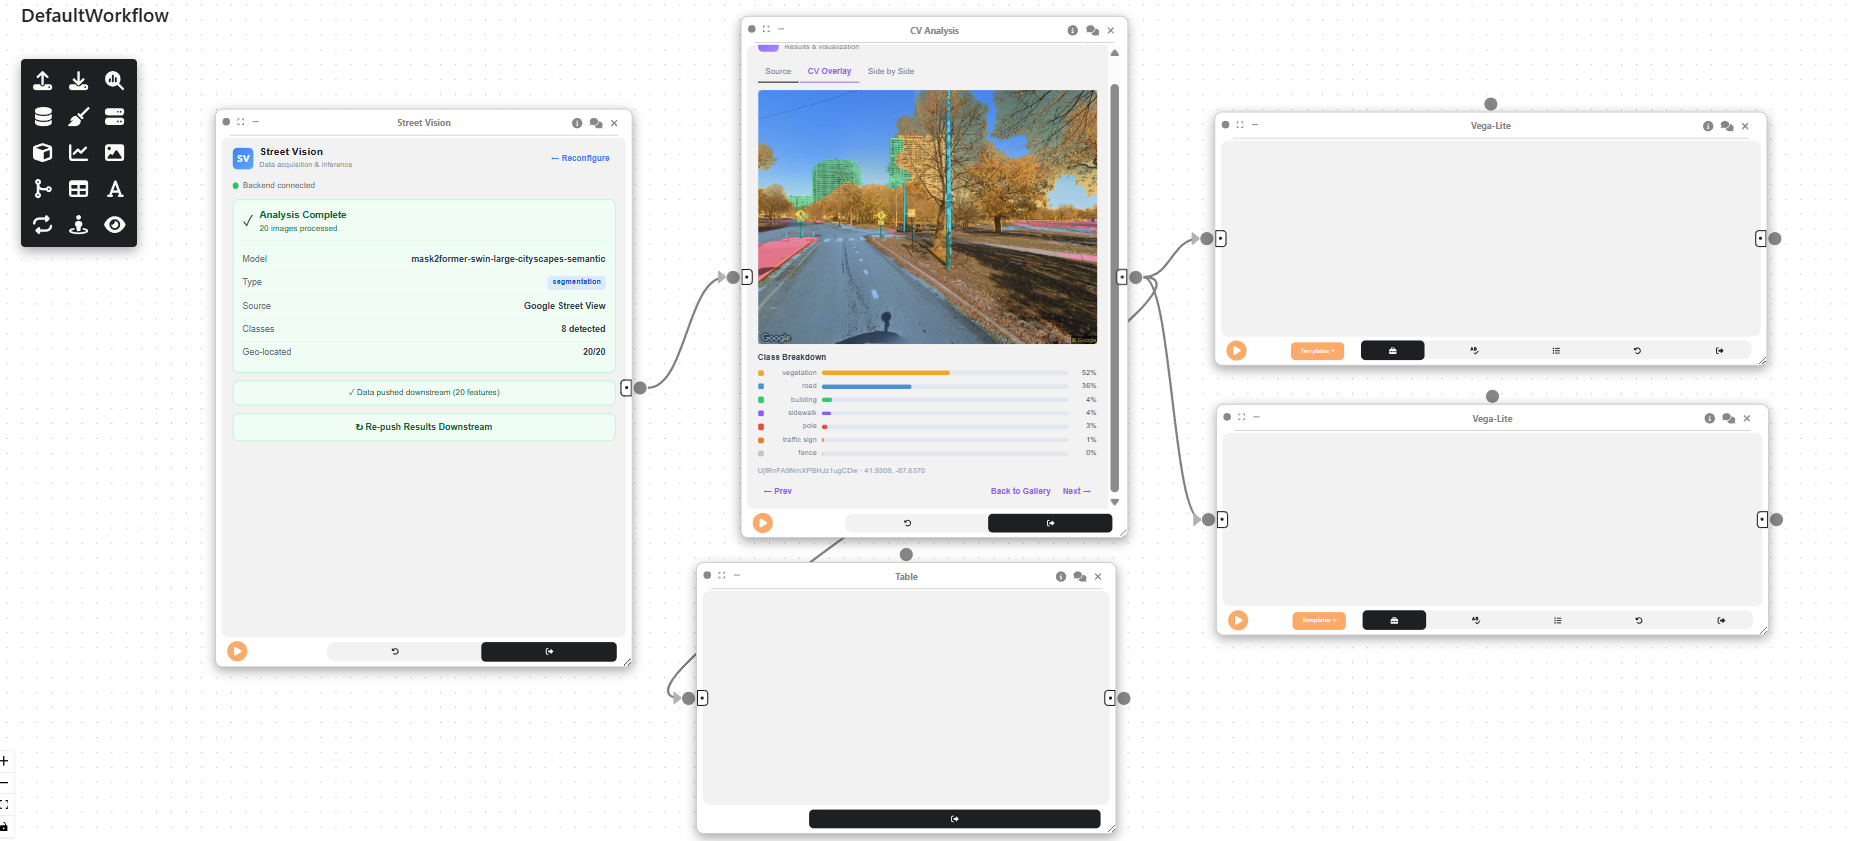
\includegraphics[width=\textwidth, alt={The CV Analysis node expanded inside the Curio canvas, with the Image Inspector open showing a Lincoln Park Street View photograph overlaid by a Mask2Former segmentation, alongside a Class Breakdown bar chart listing per-class pixel percentages.}]{gallery_inspector}
  \caption{The CV Analysis node's Image Inspector inside the Curio canvas. A Lincoln Park Street View image is shown with the Mask2Former-Swin-Large segmentation overlay, alongside a per-class breakdown bar chart that uses the same palette as the Map View.}
  \label{fig:gallery}
\end{figure*}

\textbf{Case study 2: Vehicle counting in The Loop.} Swapping the model to \texttt{ultralytics/yolov8n} and the class chips to \{car, truck, bus, motorcycle, bicycle\}, the same node returns object-count results instead of pixel ratios; the Map View template adapts because it reads from the same per-neighborhood roll-up endpoint. This is the configuration-generality claim made concrete: zero code changes between the two case studies.

\textbf{Performance.} Per-image inference latency depends on the chosen checkpoint. SegFormer-B2 on a 4-core CPU runs at $\sim$0.30~s per image, yielding $\sim$3.3~images/s end-to-end including HTTP and post-processing. Mask2Former-Swin-Large is roughly an order of magnitude larger and was not benchmarked formally; the case studies use the standard demo batch of 20 images so a single run completes in well under a minute even on the larger checkpoint. The backend caps requests at 200 images per call, primarily to keep Google Street View API quota predictable for an interactive workflow; lifting the cap is a one-line change in \texttt{inference\_service.py} for offline runs.

\textbf{Multi-node dataflow.} The teaser figure (\autoref{fig:teaser}) shows three downstream consumers wired to CV Analysis: a Vega-Lite Map View of Chicago neighborhoods coloured by their modal Cityscapes class, a Vega-Lite Neighborhood Summary bar chart of per-neighborhood image counts coloured by dominant class, and a Table node exposing the per-image feature row (latitude, longitude, per-class ratios, dominant class, neighborhood name). UTK consumption is supported via the same GeoJSON port but is not pictured. This is the Curio value proposition we set out to honour: not a monolithic CV widget, but a CV stage that participates in the dataflow graph.

\section{Discussion}
\label{sec:discussion}

\textbf{What worked.} Splitting the pipeline across two nodes was the right call. It forced a clean serialization boundary between inference and visualization, and the GeoJSON export turned out to slot directly into Curio's existing Vega-Lite and UTK consumers with no special-casing. Pre-trained models from HuggingFace were almost always good enough; we never needed to fine-tune. Server-side spatial joins via STRtree kept the client thin and made the Map View template trivially fast.

\textbf{What was harder than expected.} Coverage estimation against the Street View Metadata API turned out to be the dominant source of UX friction, not inference latency. Many Chicago bounding boxes are unevenly covered, and a user who picks a name like ``Garfield Park'' and gets back four images out of fifty assumes the model is broken. We surface a coverage percentage in the UI to set expectations but cannot fix the underlying sparsity. The fixed Cityscapes taxonomy is also a real limit: street furniture, ramps, and seasonal phenology all sit outside the 19 classes and would need either a different checkpoint (e.g.\ open-vocabulary models like CLIPSeg or SAM) or fine-tuning.

\textbf{Limitations.} (1) The 200-image per-request cap is a quota-protection measure, not a fundamental limit; large-area sweeps still need to be issued as multiple calls and reassembled downstream. (2) Street View has known temporal sparsity in residential blocks; metric stability across runs depends on which panoramas were captured most recently. (3) Inference is CPU-only; a GPU-backed deployment is straightforward but out of scope for the deliverable. (4) The neighborhood enrichment dataset is Chicago-only; extending to other cities is a configuration change but currently undocumented.

\section{Conclusion and Future Work}
\label{sec:conclusion}

We presented a two-node Curio extension that brings pre-trained street-level CV into a no-code dataflow workflow, demonstrated on Chicago greenery and vehicle counting case studies, with seven analytical tasks documented. The natural next steps are (1) GPU-backed inference and a real scaling study, (2) integrating open-vocabulary models so the target classes are not bound to Cityscapes, (3) shipping neighborhood basemaps for additional U.S.~cities, (4) adding a custom-model upload affordance, and (5) a user study to validate the time-savings claims in \autoref{tab:tasks}.

\textbf{Code availability.} Source, demo screenshots, and reproduction scripts are at \url{https://github.com/ManeeshJupalle/Street-Level-Vision-Analytics-Node-for-Curio}.

%% if specified like this the section will be omitted in review mode
\acknowledgments{%
  We thank the CS~524 instructor and teaching staff at the University of Illinois Chicago for feedback throughout the semester, in particular the recommendation that drove the two-node split. The Curio project authors made integration straightforward by keeping the \texttt{BoxDescriptor} extension surface stable.%
}

\bibliographystyle{abbrv-doi-hyperref}
\bibliography{template}

\end{document}
